In high energy physics, searches for new exotic particles have relied on hadron colliders such as the LHC as they produce extremely high energies through proton-proton collisions. These collisions produce heavy and exotic particles with extremely short lifetime that include the top quarks and W-bosons, providing enough data to study such particles extensively. Searches beyond the SM proved to be a  challenge, or rather "unlucky", at such colliders, with little-to-no signs of SUSY or anything beyond the SM since the discovery of the Higgs. In this section, I would like to discuss briefly about the LHC and the CMS detector,understanding some important kinematic variables and how a simulation is useful in search for new physics in collider experiments.

%-------------------------------------------------------------------------%
\section{The Large Hadron Collider and CMS}
\label{sec:Detector}
Located on the border of France and Switzerland, the LHC is the current world-leading facility for collider experiments. The LHC currently operates at $ \sqrt{s}=13 \text{TeV} $, with an integrated luminosity of $137\text{fb}^{-1}$. One of the primary experimental collaboration for SUSY phenomena is the CMS (Compact Muon Solenoid) \cite{chatrchyan2008cms} collaborations, where they work independently to ATLAS (A Toroidal LHC ApparatuS) \cite{collaboration2008atlas}, the other experimental collaboration searching for SUSY.  Each detector is built slightly differently to support any discoveries made at the LHC. Detectors measure energy of the deposited particles as well as their longitudinal and azimuthal components. The azimuthal component, $\phi$, covers the range of $-\pi < \phi < \pi$. The longitudinal component is known as the pseudorapidity\footnote{Also referred to as the "forward" and "backward" direction.}, an angular measure of a particle in the detector relative to the beam axis given by
\begin{equation}
    |\eta|=-\ln\Big(\tan(\frac{\theta}{2})\Big)
    \label{eq:eta}
\end{equation}
Here, $\theta$ is the polar angle between the positive direction of the beam axis and the particle's three-momentum \textbf{p}\footnote{The relationship between $\theta$ and $\eta$ being $\theta = \pm \pi/2 \rightarrow \eta = 0$, and $\theta = 0(\pi) \rightarrow \eta = +(-) \infty$}. This is measured instead of the polar angle due to the particles resulting from the collision travelling close to the speed of light and asre highly energetic. \\

The CMS detector \cite{chatrchyan2008cms} is a single large superconducting solenoid that produces 4T, surrounded by several detectors with varying purpose as shown in Figure \ref{fig:detector}. Inside the solenoid exists an inner silicon track\footnote{Highly energetic charged particles leave a trail of ionised atoms, allowing highly precise and efficient measurements of the trajectories called \textit{tracks}. Secondary vertices of the emerging particles can also be reconstructed with high precision \cite{chatrchyan2008cms}.}, electromagnetic calorimeters (ECALs) that cover the range $|\eta|<3.0$ and hadron calorimeters (HCALs) covering identical ranges. Additional forward calorimeters within the detector provides further coverage of up to $|\eta|=5$. Stable particles such as, but not limited to, the electron, photons and proton are detected by processes known as \textit{showers}. Showers occur when produced particles interact with atoms with high energies. Highly energetic muons, however, tend to escape the ECALs due to their larger mass compared to that of electrons. Thus muon chambers are required to detect outgoing muons in the form of ionisation, similarly to the inner tracks.  A quick summary of the functionality of the calorimeters are given below. \\

\begin{figure}[htbp]
    \centering
    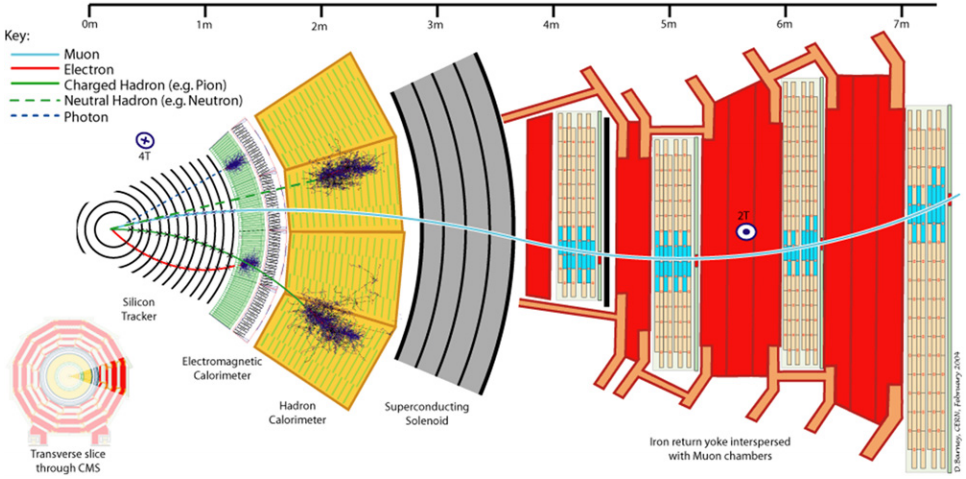
\includegraphics[width=\linewidth]{CMS_detector.png}
    \caption{A sliced view of the CMS detector, courtesy of \cite{ATLASandCMSDetector}. From left to right, we have the silicoln track to observe the motion of the charged particles heading toward the subsequent layers of the ECALs and HCALs. The calorimeters are surrounded by the 4T superconducting solenoid, also surrounded by subsequent layers of muon chambers to detect the escaping muons.}
    \label{fig:detector}
\end{figure}

\begin{itemize}
  \item \textbf{ECALs}: \par
  The ECALs measure electromagnetic showers that begin with highly energetic electrons. The electrons entering the ECALs produce energetic photons in a process known as Bremsstrahlung, which then further produces an $e^{-}e^{+}$ pair. This process is repeated in the form of a shower until there is not enough energy remaining in the photons or electrons, thus interacting with atoms in the ECAL in processes such as ionisation and scintillation \cite{thomson2013modern}. The CMS detector uses lead-tungstate ($\text{PbWO}_4$) crystals due to its high density and short radiation length. The compact size allows the showers to be contained in a confined region \cite{chatrchyan2008cms}. 
  
  \item \textbf{HCALs}: \par
  The HCALs measure hadronic jets that originate from quarks produced in the collision, and the missing energy resulting from undetectable particles such as neutrinos and other exotic particles e.g. neutralinos. The nuclear interaction between the hadrons and atoms that form the HCAL layers prompt decays of these hadronic jets through ionisation and strong interactions. The resultant particles then pass through the remaining layers interacting with the materials, thus forming showers \cite{thomson2013modern}. The CMS has focused on an alternating-layer structure with brass absorbers and plastic fluorescent scintillators. \par
  
  It is also worth noting that it is possible to identify jets originating from $b$-quarks known as \textit{b-tagging}. Due to their relatively longer lifetime, the $b$-quarks decay at a slight distance away from the collision point (primary vertex), producing a secondary vertex that is resolved when $b$-tagging \cite{thomson2013modern}. As a result, $b$-jets are identified, although the efficiency is not as high as when identifying isolated leptons. 
\end{itemize}




%-------------------------------------------------------------------------%
\section{Kinematic variables in collider experiments}
Many of the collected data at the LHC measures the properties of resultant particles and are reconstructed as a measure in the transverse plane to the beam direction. This is due to many highly energetic particle being boosted along the beam axis, making it difficult to measure components such as its energy or momentum. Considering the beam direction to be the z-direction the transverse plane would be the $(x,y)$-plane, with the geometry of this depicted in Figure \ref{fig:beam}. \\

\begin{figure}[htbp]
    \centering
    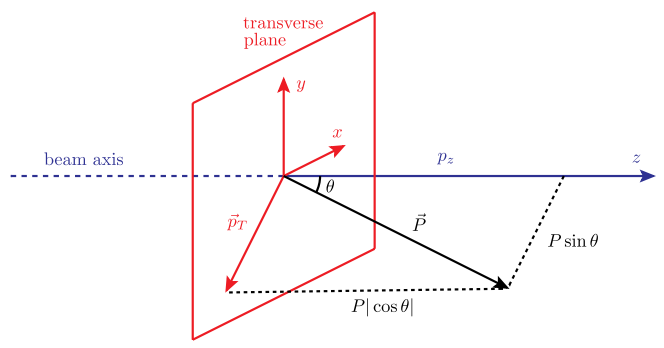
\includegraphics[width=12cm, height= 6cm]{beam.png}
    \caption{The geometry of a collider experiment, with the beam axis considered as the z-direction and the transverse plane as the $(x,y)$-plane \cite{barr2011guide}. The pseudorapidity (\ref{eq:eta}) measures the polar angle and the azimuthal component $\phi$ is parallel to the $(x,y)$-plane covering $-\pi < \phi < \pi$. }
    \label{fig:beam}
\end{figure}

One important measure is the transverse momentum, $p_T$, given by Equation (\ref{eq:pt}), 
\begin{equation}
    p_T = \abs{\overrightarrow{p_T}} = \abs{\sqrt{\overrightarrow{p_x}^2 + \overrightarrow{p_y}^2}}
    \label{eq:pt}
\end{equation}
where other important quantities can be further derived. Discriminating background and signal events in collider experiments use such quantities. These include the \textit{missing transverse energy} denoted as $\cancel{\it{E}}_{T}$, and the \textit{scalar transverse energy}\footnote{Otherwise known as the transverse hadronic energy sum.} denoted as $H_T$, given in Equation (\ref{eq:MET}) and Equation (\ref{eq:HT}), respectively. We will refer to the missing transverse energy as missing energy or MET, and the scalar transverse energy as scalar energy or HT from hereon. The missing energy of the processes are found through summing over the absent energy from the detected particles due to conservation of energy and momentum, and the scalar energy is given by the magnitude of the total energy deposited by hadronic jets. \\
\begin{equation}
    \cancel{\it{E}}_{T} = \abs{\overrightarrow{\cancel{\it{E}}_{T}}} = \abs{- \sum_i \overrightarrow{p_T}(i)}
    \label{eq:MET}
\end{equation}
\begin{equation}
    H_T = \sum_i \abs{p_T(i)} 
    \label{eq:HT}
\end{equation}

In the SM decays, leptonic final states of the top quarks produce their neutrino counterparts that freely passes through the detector, resulting in some $\cancel{\it{E}}_{T}$. Many SUSY events are predicted to have a large excess of $\cancel{\it{E}}_{T}$ more so than the SM processes, due to a larger excess of undetectable particles.  \\ 


%-------------------------------------------------------------------------%
\section{Simulations of a collider}
\label{sec:Sims}
Data collected in colliders do not initially contain a label regarding which physical process the entry corresponds to. By performing simulations identical to the parameters of the particle collider and properties closely following the production process with known theory and calculations, one may identify the existence of, or the lack of, the process of interest in the raw data through statistical techniques. There are typically three stages a collider experiment: the production/generation of the events through $pp$ collisions, the hadronisation of quarks leading to parton showers, and finally, the detection of electrons, muons, photons and jets as listed in Section \ref{sec:Detector}. \\

The generator level simulation of choice was MadGraph5\_aMC@NLO \cite{alwall2014automated} (MadGraph or MG5) due to its simplicity and fully-automated chain of simulations leading to the detector output. MadGraph calculates the cross-sections of the events of interest at leading-order (LO). However, the events do not mimic an output of the detector exactly and to achieve a high resolution of detector simulations, these events must be processed further into what a real detector may observe. The intermediate steps such as hadronization of the quarks and their showers is governed by PYTHIA8.2 \cite{sjostrand2015introduction}, integrated into MadGraph, through Monte Carlo simulations,. They include features such as \textit{multi-parton interactions} although this feature is not necessarily relevant in the analysis of our processes, thus minimizing computation time by turning it off. The output created by PYTHIA (HepMC files) may directly be fed into a detector level simulation of choice. \\

Delphes3 \cite{de2014delphes} is the detector level simulation chosen for this project due to its MG5 build-in, making the simulation process a single chain of operation following Pythia runs. The CMS detector card was chosen due to our parameters following those of CMS experiments \cite{cms2019search, cms2016searches, cms2017search}. Delphes propagates the processes generated by MadGraph and Pythia, where jets are found through the FastJet finder \cite{cacciari2012fastjet} applying the anti-$k_t$ algorithm \cite{cacciari2008anti}, to the calorimeters\footnote{See Section \ref{sec:Detector}.}. These are detected by the desired efficiencies thus the output, as a consequence, is a smeared calculation to the particle properties, in which isolated leptons, photons, jets and $\cancel{\it{E}}_{T}$ are some of the main components that are reconstructed. Other information such as the track and vertices are also calculated. The efficiencies chosen are listed in Table \ref{tab:efficiencies}, where a lepton is considered to be isolated when it remains within a cone radius of $\Delta R <0.2$ and satisfies $I(l)<0.1$, given by Equation (\ref{eq:iso}) \cite{de2014delphes}. \\

\begin{table}[htbp]
    \centering
    \begin{tabular}{c|c}
    \toprule
    Particle Type & Efficiency \\
    \midrule
    \rowcolor{gray!6} Electrons & $\abs{\eta} < 1.442$, $p_T > 20\text{ GeV}$ @ $85\%$, $\Delta R <0.2$, $I(l) <0.1$\\
    Muons & $\abs{\eta} < 2.4$, $p_T > 20\text{ GeV}$ @ $95\%$, $\Delta R < 0.2$, $I(l) <0.1$\\
    \rowcolor{gray!6} Jets & $p_T>30$ GeV, $\Delta R = 0.4$\\
    b-tagging & $60\%$ \\
    \bottomrule
    \end{tabular}
    \caption{Chosen efficiencies for our detector simulation. The isolated electrons are 10\% less efficiently identified than isolated muons, also covering a narrower $\eta$ range. The isolation variable defined by Equation (\ref{eq:iso}) determines which charged electrons and muons from the detected particles are isolated, given a minimum $p_T$ of 20 GeV. The jets have a cone size of $\Delta R = 0.4$ travelling with $p_T>30$ GeV, where 60\% of those originating from $b$-quarks are tagged correctly.} 
    \label{tab:efficiencies}    
\end{table}

\begin{equation}
    \left. I(l) = \sum\limits_{i\ne l}^{R<\Delta R} p_T(i) \middle/ p_T(l) \right. \\
    \label{eq:iso}
\end{equation}


For the purpose of this project we stick to the components listed in Table \ref{tab:variables}, including $H_T$, where leptons up to second order and jets up to fourth order are selected. In addition, each of the jets will have an associated entry as to whether it is b-tagged or not. These information will be important to our analysis in the upcoming section. \\ 


\begin{table}[htbp]
    \centering
    \begin{tabular}{c|c|c|c} 
    \toprule
     & $\cancel{\it{E}}_{T}$ & $l^{\pm}_{i=1,2}$ & $j_{i=1,2,3,4}$ \\
    \midrule
    \rowcolor{gray!6} Energy & $\abs{\cancel{\it{E}}_{T}}$ & $ p_{T_l} $ & $ p_{T_j} $ \\
    $\eta$ & $\eta_{\cancel{\it{E}}_{T}}$ & $ \eta_l $ & $ \eta_j $ \\
    \rowcolor{gray!6} $\phi$ & $\phi_{\cancel{\it{E}}_{T}}$ & $ \phi_l $ & $ \phi_j $ \\
     %&  & $  $ & $  $\\
    \bottomrule
    \end{tabular}
    \caption{The variables extracted are the energy, $\phi$ and $\eta$ components of the MET, two charged leptons (one of which is a veto), and the four jets with a minimum of one $b$-tag were chosen.} 
    \label{tab:variables}
\end{table}

%-------------------------------------------------------------------------%
\section{Cut-based searches}
\label{sec:cut}
An intuitive approach to analysing data from collider experiments have been cut-based analysis, where events are accepted or rejected based on physically motivated criteria. The objective of this method remains the same: to discriminate signal against background events and increase the signal's sensitivity. An example diagram is depicted in Figure \ref{fig:cut_flow}, where varying criterion such as $x>a$, $y>c$ and a multivariate variable $f(x,y)$, a combination of variables $x$ and $y$, accepts and rejects signal and background, respectively. The result would show the minimum number of background events remaining whilst retaining a significant portion of signal events.  \\

\begin{figure}[htbp]
    \centering
    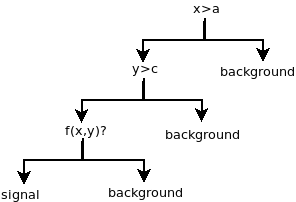
\includegraphics[width=0.5\linewidth]{cut_flow.png}
    \caption{A diagram depicting cut-flow analysis. For some criterion $x>a$, $y>c$ and a multivariate variable $f(x,y)$, the cuts accept events that satisfy such criteria, discarding events as background otherwise.}
    \label{fig:cut_flow}
\end{figure}

The benefit of such a task is that these cuts are physically well-motivated and easy to keep track of. However, this may also be a con in certain scenarios where the signatures, thus the physical properties, of the particle is not as obvious or well understood such as those in MSSM. Searches for the process $\Tilde{t}\Tilde{t}^*  \rightarrow t\bar{t}\Tilde{\chi}_1^0\Tilde{\chi}_1^0$, but not limited to, have made use of a range of variables including $\cancel{\it{E}}_{T}$, the transverse mass $M_T$, the azimuthal difference between $\cancel{\it{E}}_{T}$ and a given jet $\Delta \phi (\cancel{\it{E}}_{T}, \text{jet})$, and the number of specific particles within the data \cite{kraml2016scalar, chatrchyan2013search}. This procedure will complement machine learning algorithms that will be discussed in a later section.